\documentclass{article}
\usepackage[top=1in, bottom=1in, left=1in, right=1in]{geometry}
% \usepackage{fullpage, fancyhdr}
\usepackage{fullpage}
\usepackage{float}
\usepackage{mathtools}
\usepackage{caption}
\usepackage{subcaption}
\usepackage{portland}
\usepackage{graphicx}
%\usepackage{setspace}
\setlength{\topmargin}{0.0in}
\setlength{\headheight}{0.5in}
\setlength{\headsep}{0in}
\setlength{\footskip}{9pt}

% Use so that included code is pretty
\usepackage{listings}
\usepackage{color}

\definecolor{dkgreen}{rgb}{0,0.6,0}
\definecolor{gray}{rgb}{0.5,0.5,0.5}
\definecolor{mauve}{rgb}{0.58,0,0.82}

\lstset{ %
  backgroundcolor=\color{white},  % choose the background color; you must add \usepackage{color} or \usepackage{xcolor}
  basicstyle=\footnotesize,       % the size of the fonts that are used for the code
  breakatwhitespace=false,        % sets if automatic breaks should only happen at whitespace
  breaklines=true,                % sets automatic line breaking
  captionpos=t,                   % sets the caption-position to bottom
  commentstyle=\color{dkgreen},   % comment style
%   deletekeywords={...},           % if you want to delete keywords from the given language
%   escapeinside={\%*}{*)},         % if you want to add LaTeX within your code
%   extendedchar=false,             % lets you use non-ASCII characters; for 8-bits encodings only, does not work with UTF-8
  frame=single,                   % adds a frame around the code
  keywordstyle=\color{blue},      % keyword style
  language={[x86masm]Assembler},                % the language of the code
  morekeywords={LDR,AREA,ENTRY,CODE,DATA,DCD,SPACE,BLT,B,BL.W,ADDS,VMOV,},           % if you want to add more keywords to the set
  numbers=left,                   % where to put the line-numbers; possible values are (none, left, right)
  numbersep=5pt,                  % how far the line-numbers are from the code
  numberstyle=\tiny\color{gray},  % the style that is used for the line-numbers
  rulecolor=\color{black},        % if not set, the frame-color may be changed on line-breaks within not-black text (e.g. comments (green here))
  showspaces=false,               % show spaces everywhere adding particular underscores; it overrides 'showstringspaces'
  showstringspaces=false,         % underline spaces within strings only
  showtabs=false,                 % show tabs within strings adding particular underscores
  stepnumber=1,                   % the step between two line-numbers. If it's 1, each line will be numbered
  stringstyle=\color{mauve},      % string literal style
  tabsize=8,                      % sets default tabsize to 2 spaces
  title=\lstname                  % show the filename of files included with \lstinputlisting; also try caption instead of title
}



% \pagestyle{fancyplain}
\pagestyle{myheadings}
\voffset=-0.50in
\topmargin=0.00in 
\headsep=0.25in 
\evensidemargin=0in 
\oddsidemargin=0in 
\textwidth=6.6in 
\textheight=10.0in 

\renewcommand{\topfraction}{0.9}	% max fraction of floats at top
\renewcommand{\bottomfraction}{0.8}	% max fraction of floats at bottom
%   Parameters for TEXT pages (not float pages):
\setcounter{topnumber}{2}
\setcounter{bottomnumber}{2}
\setcounter{totalnumber}{4}     % 2 may work better
\setcounter{dbltopnumber}{2}    % for 2-column pages
\renewcommand{\dbltopfraction}{0.9}	% fit big float above 2-col. text
\renewcommand{\textfraction}{0.07}	% allow minimal text w. figs
%   Parameters for FLOAT pages (not text pages):
\renewcommand{\floatpagefraction}{0.7}	% require fuller float pages
% N.B.: floatpagefraction MUST be less than topfraction !!
\renewcommand{\dblfloatpagefraction}{0.7}	% require fuller float pages
% remember to use [htp] or [htpb] for placement

\title{Assignment \# 5: Problem Set 3}
\date{2/6/2013}
\author{Brian Arnberg}

\markright{Brian Arnberg\hfill ELEC 6260 - Embedded Computing Systems\hfill}     
\setlength{\parindent}{0pt}


\begin{document}\label{start}

% \begin{titlepage}
	\maketitle
	\thispagestyle{empty}
% \end{titlepage}


\section*{Problem 1}
Practice writing and using subroutines by writing a subroutine that calculates\\
Z = (a0 * x0) - (a1 * x1).\\

The values of the four variables a0, a1, x0, x1 are to be passed to the subroutine in
registers. The address of variable Z is to be passed to the subroutine in a register.\\

The "main" program is to call the subroutine two times, once for each of the following
sets of data. You may not use "immediate" data � all values are to be read from memory
and results are to be stored in memory.\\

x0 and x1 are to be 32-bit integers.
a0, a1, and z are to be stored using Q24.8 format.\\


First call: x0=200, x1=100, a0=5.25, a1=6.75.
Store the answer at variable z1.\\

Second call: x0=300, x1=200, a0=3.5, a1=4.125.
Store the answer at variable z2.\\

For convenience, define the arguments to be passed to the subroutine at the end of your
code section, and the variables to be written in a data section. There should be eight
"variables" in the code section � two sets of four arguments. There should be two
variables in the data section.\\

You can test this with the simulator, but version to be submitted must be executed in
RAM on the Discovery board. Submit a printout of your source program, and a screen
image of the debug window, with the results highlighted (circled) in a memory window.\\

\subsection*{Debugging Problem 1}
The Assembly Language program for Problem 1 is named \texttt{PS3-1.s}, and can be found in the Source Program Section at the end of this document. For the first run, the expected value of z1 is $375_{10}$. In Q24.8 format, this is 0x00017700. The value was expected to be stored at Memory Address 0x20003014. For the second run, the expected value of z2 is $225_{10}$. In Q24.8 format, this is 0x0000E100. The value was expected to be stored at Memory Address 0x20003018. \\

After the program was written and simulated, it was executed in RAM on the Discovery board. Figures~\ref{fig:PS3-1_Window} and~\ref{fig:PS3-1_Memory} show the debugging window after the program was executed in RAM on the board, with the values circled. Both figures indicate that the program for Problem 1 executed correctly because the results are correct. 

\newpage
\begin{figure}[h!]
	\centering
	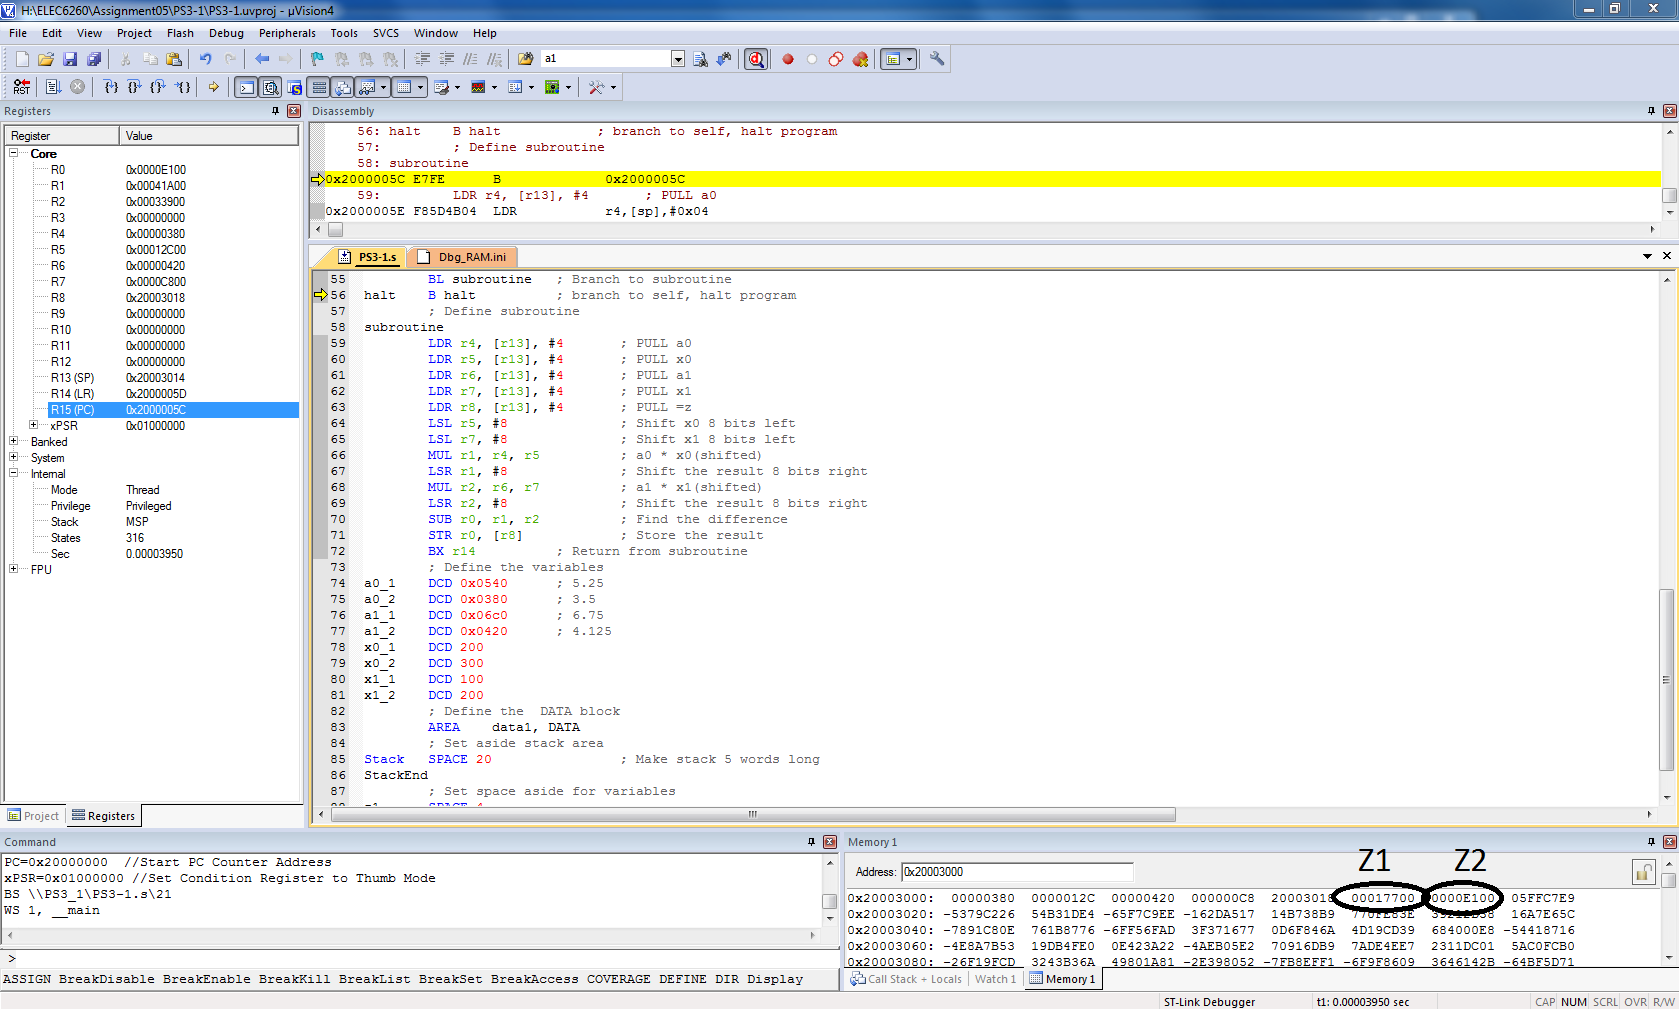
\includegraphics[width=\textwidth,keepaspectratio]{PS3-1_Window}
	\caption{A full view of the debugging window for Problem 1. The values for z1 and z2 are circled. z1 is 0x00017700 and z2 is 0x0000E100. These values are correct, so one can see that the program executed correctly.}
	\label{fig:PS3-1_Window}
\end{figure}
\begin{figure}[h!]
	\centering
	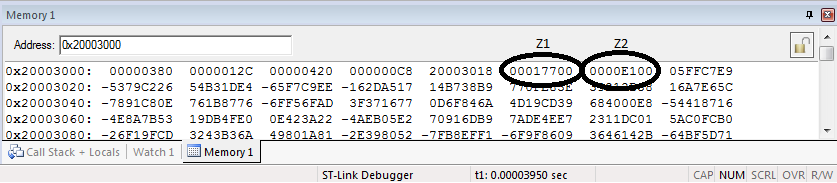
\includegraphics[width=\textwidth,keepaspectratio]{PS3-1_Memory}
	\caption{A view of the memory window for Problem 1 after the program was executed. As stated in Figure~\ref{fig:PS3-1_Window}, the values for z1 and z2 are 0x00017700 and 0x0000E100, respectively. These are the expected values, and the occur at the expected locations, so one can conclude that the program written for Problem 1 executed correctly.}
	\label{fig:PS3-1_Memory}
\end{figure}


\newpage
\section*{Problem 2}
Given below is a C program that includes several functions calls. 
\renewcommand{\labelenumi}{(\alph{enumi})}
\begin{enumerate}
	\item Write the equivalent routines in ARM assembly language and test the program in the
   Keil debugger. Submit two screen captures of the debug window, showing the final
   result returned for each of the two functions called by the main program. The main
   program and the three ``functions'' should be implemented as separate
   routines/subroutines as listed (i.e. do not "merge" them to optimize the program.)
	\item Enter and compile the C program, as given, and compare the "listing file" to your
   hand-written assembly language program. Alternatively, you may view the
   disassembled code in the debugger window to see the C and equivalent assembly
   language instructions. Turn off any optimizations that would normally be performed
   by the C compiler.
\end{enumerate}

\begin{lstlisting}[language=C, frame=none, numbers=none ]
	int k;      //global variable

	int f1(int x1, int x2) {
	    return x1 + x2;
	}

	int f2(int x1) {
	    return x1 + 1;
	}

	void f3(int r) {
	    int j;
	    for (j = 0; j < 2; j++)
	            k = k + f1(r + j, 5);
	}
	
	void main () {
	    int a;
	    k = 0;
	    f3(3);
	    a = f2(2);
	}
 \end{lstlisting}
 \subsection*{Problem 2, part (a) }
 The ARM assembly language program that emulates the above C program was written and named \texttt{PS3-2.s}. The program can be found in the Source Programs section at the end of this document. The program was tested in the Keil debugger. Figure~\ref{fig:PS3-2_f3} displays the memory on the board after \texttt{f3} was called, and Figure~\ref{fig:PS3-2_f2} displays the memory on the board after \texttt{f2} was called. Both figures display the expected values for the final result returned for each of the two functions called by the main program, so it can be observed that the hand-written program works correctly. 
\begin{figure}[htbp]
	\centering
	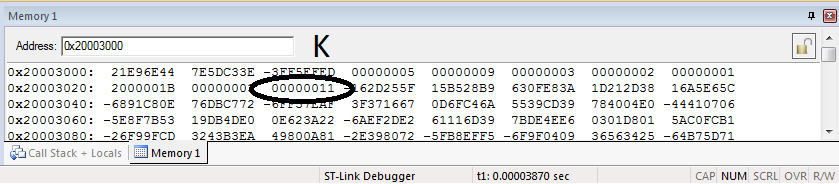
\includegraphics[width=\textwidth,keepaspectratio]{PS3-2_f3}
	\caption{A view of the memory window after the main function in Problem 2 calls \texttt{f3}. The circled value is the value for k, 0x00000011, which corresponds to the expected result, $17_{10}$. This means that the program executed \texttt{f3} and \texttt{f1} correctly.}
	\label{fig:PS3-2_f3}
\end{figure}
\begin{figure}[htbp]
	\centering
	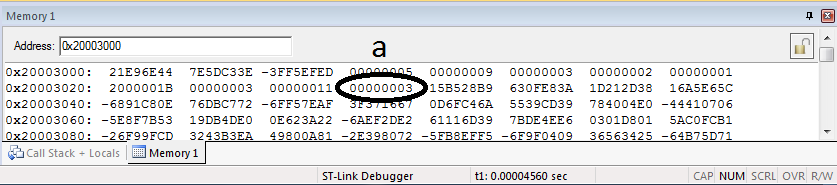
\includegraphics[width=\textwidth,keepaspectratio]{PS3-2_f2}
	\caption{A view of the memory window after the main function in Problem 2 calls \texttt{f2}. The circle value is the value for a, 0x00000003, which corresponds to the expected result, 3. This means that the program executed \texttt{f2} correctly.}
	\label{fig:PS3-2_f2}
\end{figure}

\newpage
\subsection*{Problem 2, part (b) }
The C program listed above was entered and compiled, as given. All compiler optimizations were turned off. Then, it was debugged on the Discovery board so that the disassembled code could be used to compare the compiler output to my hand-written assembly language program. A section of the disassembled code was copied into \texttt{PS3-2b.txt}, which can be found in the Source Programs section at the end of this document.
\\

The hand-written program was greater than 60 lines of assembly, while the disassembled code was just over 30 lines of assembly. This means that the C program, once disassembled, was approximately twice as fast as the hand-written program. The line length difference can be attributed, at least in part, to the way the C program treated certain register values as constants. Additionally, the hand-written code interacted with the stack value by value (\texttt{STR r1, [r13, \#-4]!}), while the C program disassembled to use \texttt{PUSH} and \texttt{POP}.  Also, the disassembled code was simply more elegant, even without any optimizations. 

\section*{Conclusions}
Both ARM assembly language programs written were functionally correct. Each program was executed on the Discovery board, and each program returned expected values. The C program, when disassembled, was more efficient than the hand-written program. 
\newpage
\section*{ Source Programs }
\lstinputlisting{PS3-1.s}
\newpage
\lstinputlisting{PS3-2.s}
\lstinputlisting[numbers=none]{PS3-2b.txt}



%  \begin{figure}[htbp]
%   \centering
%   \includegraphics[width=4.0in,keepaspectratio]{E-Field}
%   \caption{\small{ The E-Field pattern produced by the initial code. }}
%   \label{fig:E-Field}
%   \end{figure}
%  \begin{figure}[htbp]
%   \centering
%   \includegraphics[width=4.0in,keepaspectratio]{Power}
%   \caption{\small{ The normalized power pattern of the system.  }}
%   \label{fig:Power}
%   \end{figure}

\label{end}\end{document}


